% Options for packages loaded elsewhere
\PassOptionsToPackage{unicode}{hyperref}
\PassOptionsToPackage{hyphens}{url}
\PassOptionsToPackage{dvipsnames,svgnames,x11names}{xcolor}
%
\documentclass[
  11pt,
]{article}

\usepackage{amsmath,amssymb}
\usepackage{iftex}
\ifPDFTeX
  \usepackage[T1]{fontenc}
  \usepackage[utf8]{inputenc}
  \usepackage{textcomp} % provide euro and other symbols
\else % if luatex or xetex
  \usepackage{unicode-math}
  \defaultfontfeatures{Scale=MatchLowercase}
  \defaultfontfeatures[\rmfamily]{Ligatures=TeX,Scale=1}
\fi
\usepackage{lmodern}
\ifPDFTeX\else  
    % xetex/luatex font selection
\fi
% Use upquote if available, for straight quotes in verbatim environments
\IfFileExists{upquote.sty}{\usepackage{upquote}}{}
\IfFileExists{microtype.sty}{% use microtype if available
  \usepackage[]{microtype}
  \UseMicrotypeSet[protrusion]{basicmath} % disable protrusion for tt fonts
}{}
\makeatletter
\@ifundefined{KOMAClassName}{% if non-KOMA class
  \IfFileExists{parskip.sty}{%
    \usepackage{parskip}
  }{% else
    \setlength{\parindent}{0pt}
    \setlength{\parskip}{6pt plus 2pt minus 1pt}}
}{% if KOMA class
  \KOMAoptions{parskip=half}}
\makeatother
\usepackage{xcolor}
\usepackage[top=1in,bottom=1in,left=1.25in,right=1.25in]{geometry}
\setlength{\emergencystretch}{3em} % prevent overfull lines
\setcounter{secnumdepth}{5}
% Make \paragraph and \subparagraph free-standing
\makeatletter
\ifx\paragraph\undefined\else
  \let\oldparagraph\paragraph
  \renewcommand{\paragraph}{
    \@ifstar
      \xxxParagraphStar
      \xxxParagraphNoStar
  }
  \newcommand{\xxxParagraphStar}[1]{\oldparagraph*{#1}\mbox{}}
  \newcommand{\xxxParagraphNoStar}[1]{\oldparagraph{#1}\mbox{}}
\fi
\ifx\subparagraph\undefined\else
  \let\oldsubparagraph\subparagraph
  \renewcommand{\subparagraph}{
    \@ifstar
      \xxxSubParagraphStar
      \xxxSubParagraphNoStar
  }
  \newcommand{\xxxSubParagraphStar}[1]{\oldsubparagraph*{#1}\mbox{}}
  \newcommand{\xxxSubParagraphNoStar}[1]{\oldsubparagraph{#1}\mbox{}}
\fi
\makeatother


\providecommand{\tightlist}{%
  \setlength{\itemsep}{0pt}\setlength{\parskip}{0pt}}\usepackage{longtable,booktabs,array}
\usepackage{calc} % for calculating minipage widths
% Correct order of tables after \paragraph or \subparagraph
\usepackage{etoolbox}
\makeatletter
\patchcmd\longtable{\par}{\if@noskipsec\mbox{}\fi\par}{}{}
\makeatother
% Allow footnotes in longtable head/foot
\IfFileExists{footnotehyper.sty}{\usepackage{footnotehyper}}{\usepackage{footnote}}
\makesavenoteenv{longtable}
\usepackage{graphicx}
\makeatletter
\def\maxwidth{\ifdim\Gin@nat@width>\linewidth\linewidth\else\Gin@nat@width\fi}
\def\maxheight{\ifdim\Gin@nat@height>\textheight\textheight\else\Gin@nat@height\fi}
\makeatother
% Scale images if necessary, so that they will not overflow the page
% margins by default, and it is still possible to overwrite the defaults
% using explicit options in \includegraphics[width, height, ...]{}
\setkeys{Gin}{width=\maxwidth,height=\maxheight,keepaspectratio}
% Set default figure placement to htbp
\makeatletter
\def\fps@figure{htbp}
\makeatother
% definitions for citeproc citations
\NewDocumentCommand\citeproctext{}{}
\NewDocumentCommand\citeproc{mm}{%
  \begingroup\def\citeproctext{#2}\cite{#1}\endgroup}
\makeatletter
 % allow citations to break across lines
 \let\@cite@ofmt\@firstofone
 % avoid brackets around text for \cite:
 \def\@biblabel#1{}
 \def\@cite#1#2{{#1\if@tempswa , #2\fi}}
\makeatother
\newlength{\cslhangindent}
\setlength{\cslhangindent}{1.5em}
\newlength{\csllabelwidth}
\setlength{\csllabelwidth}{3em}
\newenvironment{CSLReferences}[2] % #1 hanging-indent, #2 entry-spacing
 {\begin{list}{}{%
  \setlength{\itemindent}{0pt}
  \setlength{\leftmargin}{0pt}
  \setlength{\parsep}{0pt}
  % turn on hanging indent if param 1 is 1
  \ifodd #1
   \setlength{\leftmargin}{\cslhangindent}
   \setlength{\itemindent}{-1\cslhangindent}
  \fi
  % set entry spacing
  \setlength{\itemsep}{#2\baselineskip}}}
 {\end{list}}
\usepackage{calc}
\newcommand{\CSLBlock}[1]{\hfill\break\parbox[t]{\linewidth}{\strut\ignorespaces#1\strut}}
\newcommand{\CSLLeftMargin}[1]{\parbox[t]{\csllabelwidth}{\strut#1\strut}}
\newcommand{\CSLRightInline}[1]{\parbox[t]{\linewidth - \csllabelwidth}{\strut#1\strut}}
\newcommand{\CSLIndent}[1]{\hspace{\cslhangindent}#1}

\makeatletter
\@ifpackageloaded{caption}{}{\usepackage{caption}}
\AtBeginDocument{%
\ifdefined\contentsname
  \renewcommand*\contentsname{Table of contents}
\else
  \newcommand\contentsname{Table of contents}
\fi
\ifdefined\listfigurename
  \renewcommand*\listfigurename{List of Figures}
\else
  \newcommand\listfigurename{List of Figures}
\fi
\ifdefined\listtablename
  \renewcommand*\listtablename{List of Tables}
\else
  \newcommand\listtablename{List of Tables}
\fi
\ifdefined\figurename
  \renewcommand*\figurename{Figure}
\else
  \newcommand\figurename{Figure}
\fi
\ifdefined\tablename
  \renewcommand*\tablename{Table}
\else
  \newcommand\tablename{Table}
\fi
}
\@ifpackageloaded{float}{}{\usepackage{float}}
\floatstyle{ruled}
\@ifundefined{c@chapter}{\newfloat{codelisting}{h}{lop}}{\newfloat{codelisting}{h}{lop}[chapter]}
\floatname{codelisting}{Listing}
\newcommand*\listoflistings{\listof{codelisting}{List of Listings}}
\makeatother
\makeatletter
\makeatother
\makeatletter
\@ifpackageloaded{caption}{}{\usepackage{caption}}
\@ifpackageloaded{subcaption}{}{\usepackage{subcaption}}
\makeatother
\ifLuaTeX
  \usepackage{selnolig}  % disable illegal ligatures
\fi
\usepackage{bookmark}

\IfFileExists{xurl.sty}{\usepackage{xurl}}{} % add URL line breaks if available
\urlstyle{same} % disable monospaced font for URLs
\hypersetup{
  pdftitle={SmartMatch: A Multi-Agent Pipeline for Mood Board Generation via Graph-Augmented Retrieval and Multimodal Synthesis},
  colorlinks=true,
  linkcolor={blue},
  filecolor={Maroon},
  citecolor={Blue},
  urlcolor={Blue},
  pdfcreator={LaTeX via pandoc}}

\title{SmartMatch: A Multi-Agent Pipeline for Mood Board Generation via
Graph-Augmented Retrieval and Multimodal Synthesis}
\author{Qingyang Wang \and Nandini Kodali \and Caroline
Delva \and Xinzhou Li}
\date{}

\begin{document}
\maketitle
\begin{abstract}
Visual content selection is a recurring challenge for creatives and
marketers who must identify images that match not just a topic but a
specific emotional tone, aesthetic intent, and compositional style.
Conventional image search fails because abstract or emotionally rich
language does not map naturally to the visual feature spaces that
retrieval models operate in.

We present SmartMatch, a multi-agent system that generates cohesive
nine-image mood boards from free-form natural language. The pipeline
comprises five stages: a Visual Concept Grounding Agent that uses Claude
to decompose user intent into structured visual descriptors; a Hybrid
Retrieval system combining SigLIP-2 visual embeddings with per-field
OpenAI text embeddings over 25,000 Unsplash images; a Graph RAG Agent
that builds a knowledge graph over the corpus and performs candidate
deduplication, expansion, and reranking; a Multimodal Verification and
Coherence Agent that selects a visually consistent final set; and a
Justification Agent that produces natural-language explanations for each
image alongside a board-level narrative. When retrieval scores fall
below a threshold, the system falls back to gpt-image-1 with
Claude-driven diverse prompt synthesis.

LLM-as-judge evaluation across 50 diverse queries yields an overall mean
score of 3.45 out of 5.0, with relevance at 4.18, visual quality at
3.40, coherence at 3.06, and aesthetics at 3.16. An ablation study
confirms that LLM grounding contributes the largest single gain in
relevance (+0.7) and Graph RAG the largest gain in coherence (+0.6). The
system runs entirely on consumer hardware without a GPU and is deployed
as a live Streamlit application on HuggingFace Spaces.
\end{abstract}

\section{Introduction}\label{introduction}

Selecting images for a mood board requires matching visual output to
emotional intent. A user searching for images that evoke the feeling of
being burnt out after a long week is not describing a literal scene but
expressing an affective state that should translate into a specific
palette, lighting, compositional weight, and subject matter.
Conventional image search engines fail at this translation because
vision-language models such as SigLIP-2 are trained primarily on literal
object descriptions, and emotionally rich language, abstract concepts,
and aesthetic intentions are systematically underrepresented in their
training distributions.

A system designed to bridge this gap must do more than retrieve images.
It must interpret intent, structure the retrieval problem, evaluate
coherence across a set of images, and explain its selections. SmartMatch
addresses all four requirements through a coordinated multi-agent
pipeline that produces a nine-image mood board with per-image
justifications and a board-level narrative.

The research questions motivating this work are: (1) Does LLM-based
visual grounding improve retrieval quality for abstract queries compared
to direct embedding search? (2) Does graph-augmented retrieval improve
mood board coherence compared to flat similarity search? We evaluate
both questions through an ablation study and an LLM-as-judge framework
across 50 diverse queries.

\section{Related Work}\label{related-work}

\textbf{Vision-language retrieval.} Contrastive models such as CLIP
(Radford et al. 2021) and SigLIP (Zhai et al. 2023) enable zero-shot
image retrieval through shared embedding spaces. SigLIP-2 improves on
CLIP via sigmoid loss, achieving stronger multi-label retrieval
performance. However, their text encoders favor literal descriptions
over affective language. Per-field scoring approaches (Khattab and
Zaharia 2020; Karpukhin et al. 2020) suggest that decomposing queries
into independent semantic dimensions can improve over single-vector
retrieval, an insight that informs SmartMatch's hybrid retrieval design.

\textbf{LLM-augmented retrieval.} Retrieval-Augmented Generation (Lewis
et al. 2020) and HyDE (Gao et al. 2023) demonstrate that LLMs can
reframe queries into forms better suited to retrieval models.
SmartMatch's grounding agent applies this principle by converting
abstract user text into structured visual descriptors aligned with
SigLIP-2's training distribution.

\textbf{Graph-based recommendation.} Neural graph collaborative
filtering (Wang et al. 2019) shows that item-graph connectivity is a
reliable signal for recommendation diversity. SmartMatch adapts this to
image retrieval by constructing edges based on weighted field-level
similarity across mood, color palette, and visual description.

\textbf{Mood board generation.} Prior computational approaches
(O'Donovan, Agarwala, and Hertzmann 2011; Gatys, Ecker, and Bethge 2016)
focused on color harmony and style transfer using hand-crafted features,
without support for semantic or emotional intent. SmartMatch is the
first system to combine LLM grounding, hybrid semantic retrieval,
graph-augmented reranking, and LLM-based coherence selection in a
unified mood board pipeline.

\section{System Architecture}\label{system-architecture}

SmartMatch is a multi-agent pipeline coordinated by an OrchestratorAgent
that manages routing, step timing, structured logging, and safety
checks. The system accepts free-form text and optionally uploaded
images, and returns a nine-image mood board with per-image
justifications and a board-level narrative. All inter-agent
communication uses Pydantic models rather than raw dictionaries,
ensuring field mismatches fail loudly at parse time.

\subsection{Pipeline Overview}\label{pipeline-overview}

The pipeline follows two branches. Branch A handles uploaded images:
after grounding, the system routes directly to the Generation Agent for
image editing. Branch B, the primary path, handles text-only queries
through hybrid retrieval, Graph RAG, verification, and coherence
selection. If the top retrieval score falls below a threshold of 0.5,
the system falls back to on-demand generation. The routing decision
deliberately uses the pre-Graph RAG hybrid score rather than the
post-reranking score. Graph expansion and connectivity-based reranking
can inflate scores for abstract queries by surfacing well-connected
neighbors, masking the fact that no genuinely relevant images exist in
the corpus. Using the raw hybrid score as the routing signal ensures the
generation fallback is triggered when retrieval quality is actually
insufficient.

\begin{figure}[H]

\centering{

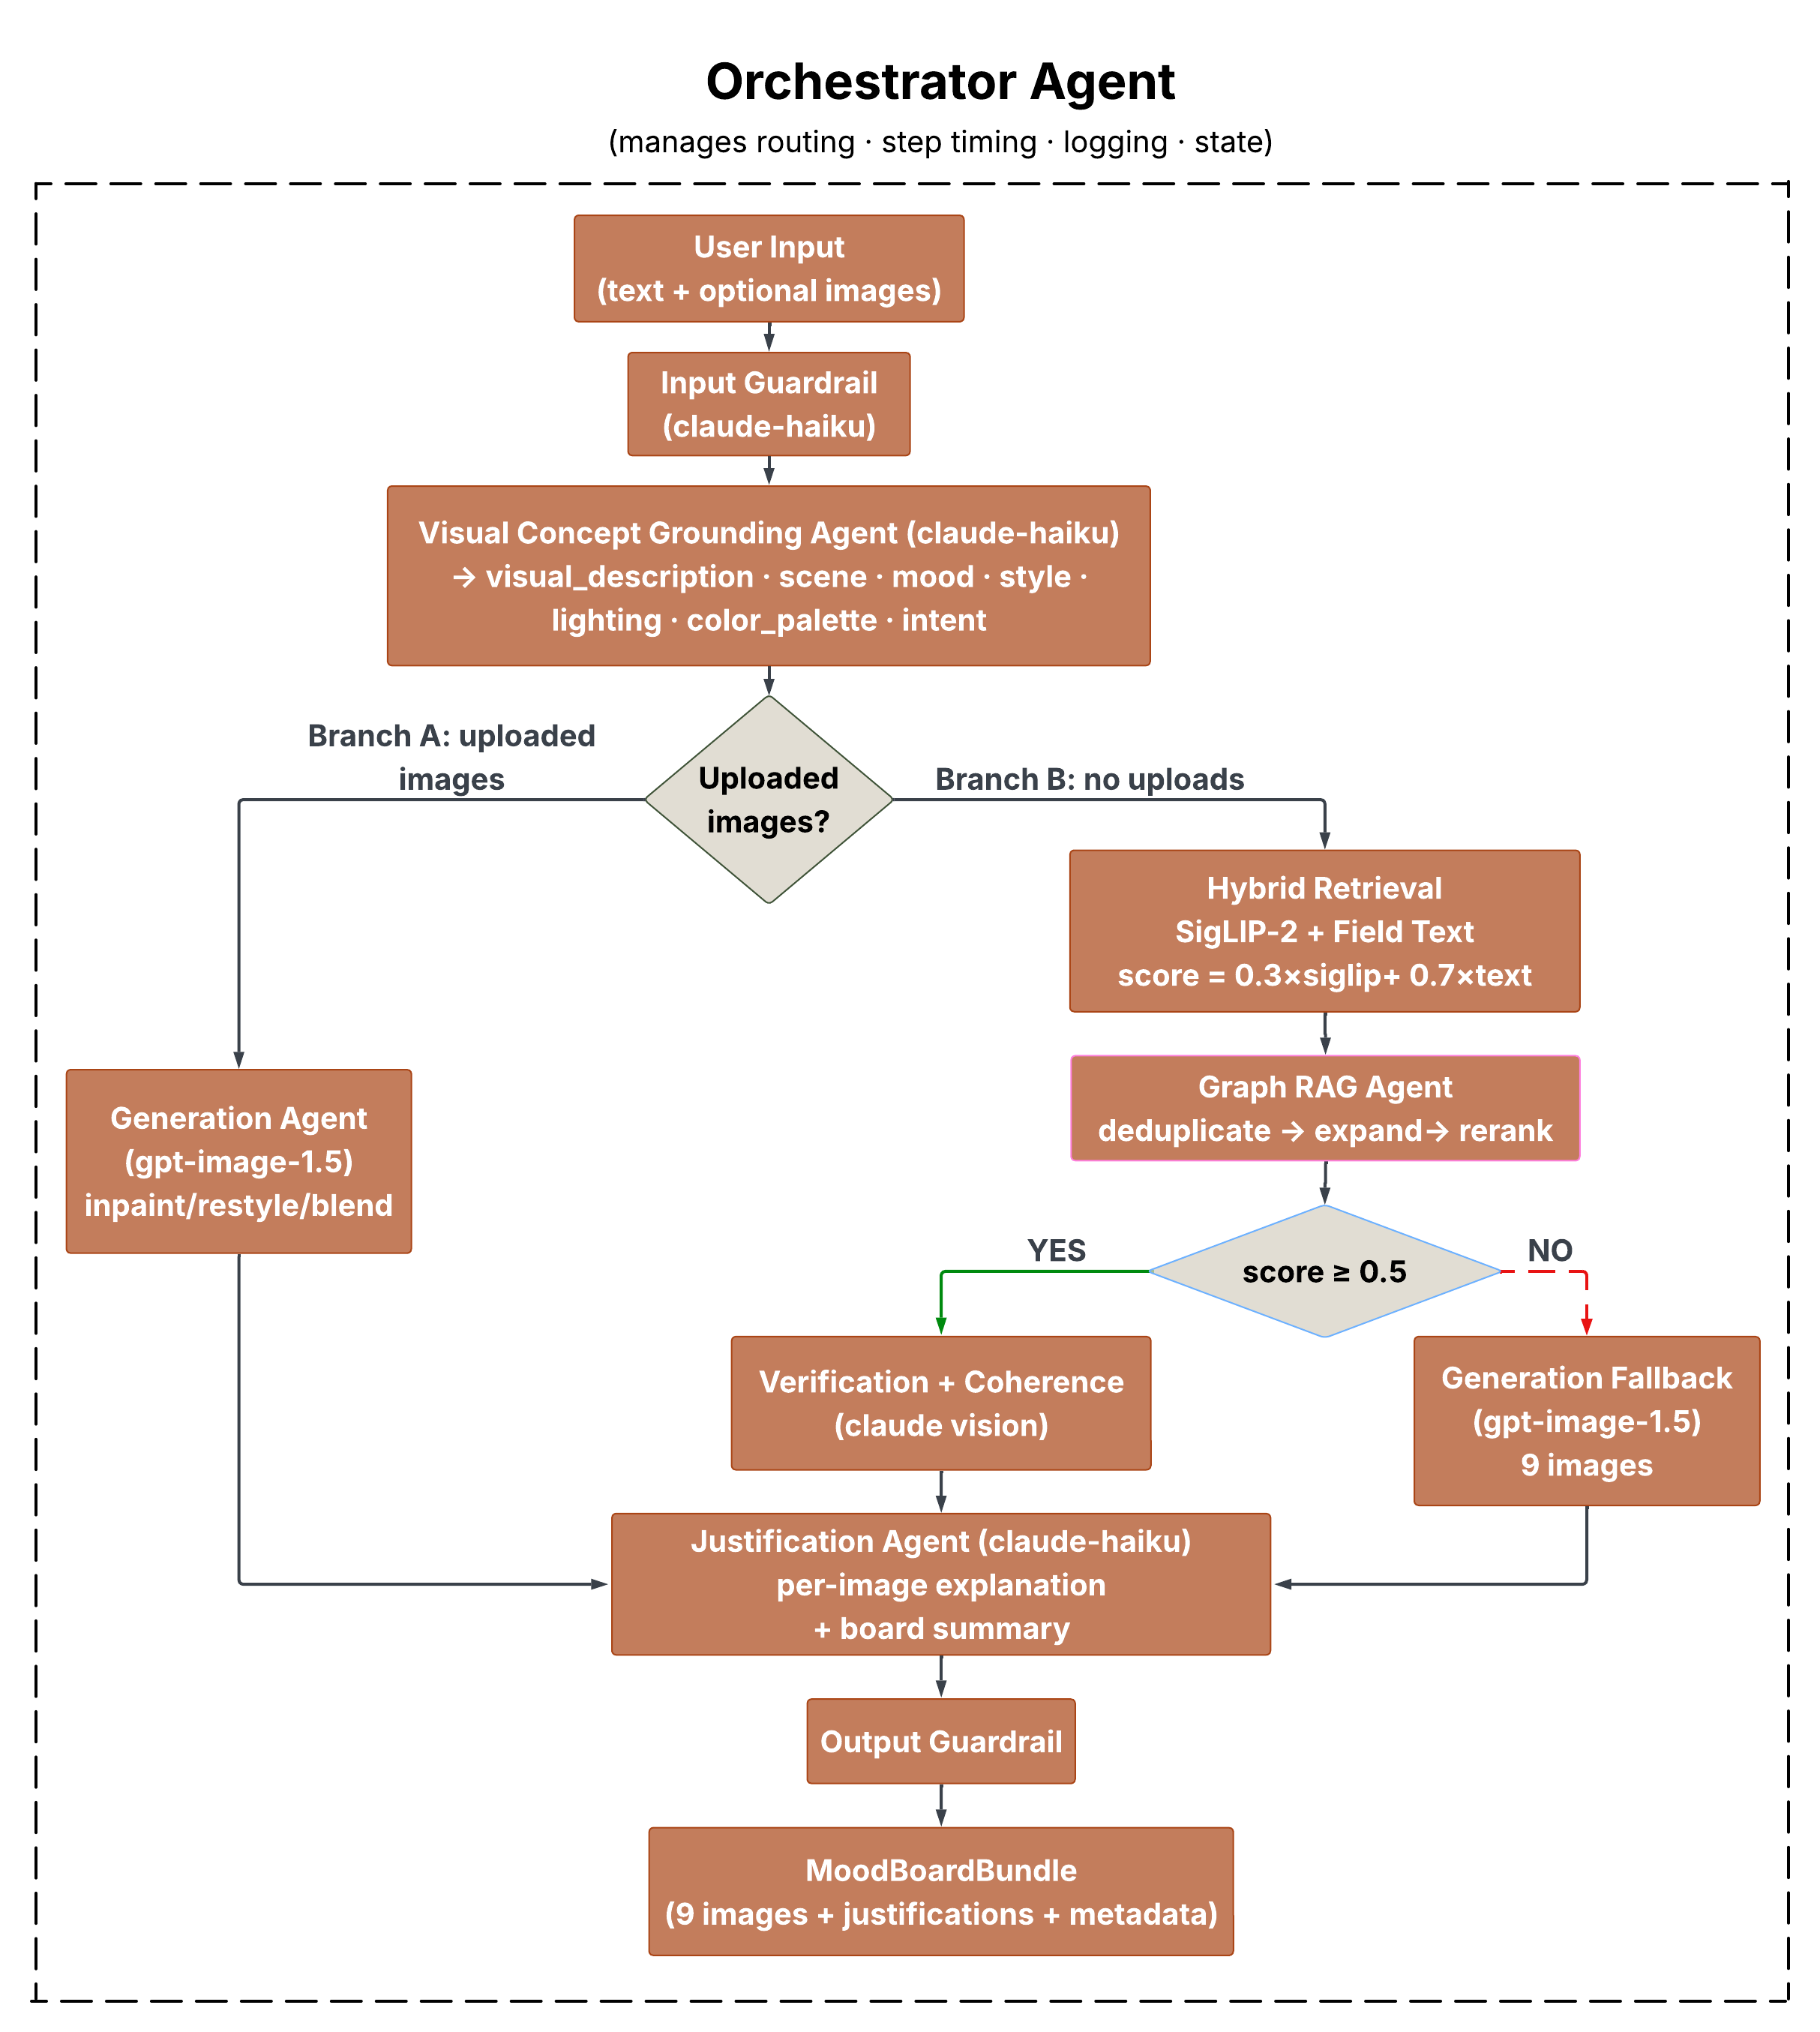
\includegraphics{images/Pipeline.png}

}

\caption{\label{fig-pipeline}SmartMatch System Architecture:
Orchestrator-coordinated multi-agent pipeline}

\end{figure}%

\subsection{Visual Concept Grounding
Agent}\label{visual-concept-grounding-agent}

The grounding agent transforms raw user text into a structured JSON
object using Claude (claude-haiku-4-5-20251001). The output contains
seven fields:

\begin{longtable}[]{@{}ll@{}}
\caption{Output fields produced by the Visual Concept Grounding
Agent}\label{tbl-grounding-fields}\tabularnewline
\toprule\noalign{}
Field & Description \\
\midrule\noalign{}
\endfirsthead
\toprule\noalign{}
Field & Description \\
\midrule\noalign{}
\endhead
\bottomrule\noalign{}
\endlastfoot
visual\_description & A rich sentence describing the ideal image \\
scene & Scene and setting keywords \\
mood & Emotional and atmospheric keywords \\
style & Visual style keywords \\
lighting & Lighting conditions \\
color\_palette & Dominant colors and tones \\
intent & Use case: professional, editorial, or social \\
\end{longtable}

The agent supports multi-turn refinement via a MemoryManager that
persists grounding outputs across turns within a session. When a user
submits a follow-up request, the new query is composed with the previous
grounding output and the full conversation history, so the system
modifies direction incrementally rather than restarting from scratch.
For example, after generating an initial board for ``feeling burnt out
after a long week,'' a follow-up of ``make it warmer and less isolated''
shifts the mood and color\_palette fields while preserving the original
scene and intent. Liked images are kept across turns; only the remaining
slots are re-retrieved or re-generated. For offline preprocessing, the
Anthropic Batch API generates grounding outputs for all 25,000 corpus
images at a 50\% cost reduction versus the live API, eliminating
per-image LLM calls from the inference path and reducing live Claude
usage to query-level grounding only.

\subsection{Hybrid Retrieval}\label{hybrid-retrieval}

Retrieval combines two complementary signals. The SigLIP-2 Retrieval
Agent performs cosine similarity search over a FAISS index of 25,000
pre-computed image embeddings using google/siglip-base-patch16-224. The
Field Text Retrieval Agent computes per-field semantic embeddings via
OpenAI text-embedding-3-large independently for visual\_description,
mood, and color\_palette. The hybrid score is:

\[\text{score} = 0.3 \times \text{siglip\_score} + 0.7 \times \text{text\_score}\]

Text similarity is weighted more heavily (0.7) because SigLIP-2 scores
are frequently negative in high-dimensional space, particularly for
abstract emotional queries. The text embedding component reliably
captures the semantic intent of the grounding output. The system
retrieves up to 20 candidates before Graph RAG processing.

\subsection{Graph RAG Agent}\label{graph-rag-agent}

An offline script builds a weighted knowledge graph over all 25,000
images using FAISS-based nearest-neighbor search per embedding field.
Edge weights are computed as a weighted combination of field-level
similarities:

\[\text{edge\_weight} = 0.35 \times \text{mood\_sim} + 0.20 \times \text{color\_sim} + 0.45 \times \text{visual\_sim}\]

This formulation connects images that share visual appearance and
atmosphere. The graph has 750,000 edges across 25,000 nodes with an
average degree of 30.

The agent operates in three steps:

\begin{enumerate}
\def\labelenumi{\arabic{enumi}.}
\tightlist
\item
  \textbf{Deduplicate}: removes candidate pairs with edge weight above
  0.60, keeping the higher-scoring image in each near-duplicate pair.
\item
  \textbf{Expand}: takes the top-5 seed candidates, traverses their
  graph neighbors, and adds up to 10 new candidates. A maximum of 2 new
  candidates are allowed per seed to ensure diversity. Expanded
  candidates are scored using real text similarity via
  \texttt{\_score\_all} rather than proxy scores, so they compete on the
  same scale as hybrid retrieval candidates.
\item
  \textbf{Rerank}: combines hybrid score and graph connectivity as
  \(\text{final} = 0.75 \times \text{hybrid} + 0.25 \times \text{connectivity}\),
  where connectivity is the average edge weight to other candidates in
  the set.
\end{enumerate}

\subsection{Multimodal Verification and
Coherence}\label{multimodal-verification-and-coherence}

The Multimodal Verification Agent passes each candidate to Claude
Vision, evaluating whether each image genuinely matches the mood,
palette, and intent of the query. If fewer than 6 images pass, the
Generation Agent fills the gap; generated images are flagged
\texttt{verified=True} so they are included in the Coherence selection
pool. The Coherence Agent receives the top 20 verified candidates and
uses Claude to select the final 9 images that best balance thematic
consistency, visual diversity, and aesthetic harmony.

\subsection{Generation Agent}\label{generation-agent}

When retrieval fails, the Generation Agent synthesizes images using
gpt-image-1. The key mechanism is Claude-driven diverse prompt
synthesis: before generation, Claude produces \(n\) visually distinct
image descriptions enforcing variation across subject type (person,
interior, outdoor, still life, abstract, urban, nature, silhouette,
aerial), scale (extreme close-up through aerial), and emotional register
(literal, symbolic, atmospheric). Each description is combined with a
distinct photographic style variant. API calls run concurrently with a
thread pool of 3 workers, reducing wall-clock time from approximately 90
seconds to 25-30 seconds. If any generated image scores below 0.15 on
the hybrid similarity measure, Claude refines that specific prompt using
the prior prompt and score as context and regenerates only that image, a
targeted quality-enforcement loop that avoids discarding the full batch
while ensuring the board meets a minimum visual standard.

\subsection{Justification Agent}\label{justification-agent}

The Justification Agent produces a 2-3 sentence per-image explanation
grounded in the image caption and user query, and a 3-5 sentence
board-level narrative. All output is generated by Claude without
reference to scores or technical details.

\subsection{Supporting Components}\label{supporting-components}

The OrchestratorAgent coordinates all stages via lazy agent
initialization. The GuardrailAgent blocks harmful queries while allowing
dark, melancholy, or unconventional creative requests, and fails open on
API error. The PipelineLogger writes structured JSONL logs capturing
step timings, routing decisions, and verification outcomes. The
Streamlit interface exposes multi-turn refinement through a persistent
chat panel: after a board is generated, users can type natural-language
feedback (e.g., ``more abstract, remove people'') which triggers
re-grounding with the accumulated conversation history, keeping liked
images and replacing the rest.

\subsection{External Services}\label{external-services}

\begin{longtable}[]{@{}
  >{\raggedright\arraybackslash}p{(\columnwidth - 2\tabcolsep) * \real{0.5000}}
  >{\raggedright\arraybackslash}p{(\columnwidth - 2\tabcolsep) * \real{0.5000}}@{}}
\caption{External services and models used by
SmartMatch}\label{tbl-external-services}\tabularnewline
\toprule\noalign{}
\begin{minipage}[b]{\linewidth}\raggedright
Component
\end{minipage} & \begin{minipage}[b]{\linewidth}\raggedright
Service
\end{minipage} \\
\midrule\noalign{}
\endfirsthead
\toprule\noalign{}
\begin{minipage}[b]{\linewidth}\raggedright
Component
\end{minipage} & \begin{minipage}[b]{\linewidth}\raggedright
Service
\end{minipage} \\
\midrule\noalign{}
\endhead
\bottomrule\noalign{}
\endlastfoot
Grounding, verification, coherence, justification, prompt synthesis &
Anthropic API (claude-haiku-4-5-20251001) \\
Image retrieval embeddings & SigLIP-2
(google/siglip-base-patch16-224) \\
Field-level text embeddings & OpenAI text-embedding-3-large \\
Fallback image generation & gpt-image-1 \\
Similarity search & FAISS \\
Image dataset & Unsplash (25,000 images) \\
Batch grounding preprocessing & Anthropic Batch API \\
\end{longtable}

\section{Data and Preprocessing}\label{data-and-preprocessing}

The image corpus consists of 25,000 photographs from the Unsplash
dataset, selected for diversity across subjects, moods, and visual
styles. Grounding outputs for all 25,000 images were generated offline
via the Anthropic Batch API. SigLIP-2 embeddings are stored in a FAISS
flat inner product index with L2 normalization. Field text embeddings
produce a 25,000 x 3,072 matrix per field stored as NumPy float32
arrays. The knowledge graph was built offline in approximately 8 minutes
on CPU using FAISS-based nearest-neighbor search per field with the
weighted combination described in the Graph RAG Agent section.

The evaluation query set consists of 50 queries manually constructed to
span five categories with 10 queries each: emotional and lifestyle,
seasonal and nature, lifestyle and aesthetic, commercial and campaign,
and abstract and conceptual. Queries were designed to vary in
specificity (concrete scenes versus affective states), vocabulary
(literal versus metaphorical), and expected corpus coverage
(well-represented versus niche). This design ensures the evaluation
captures both the system's strengths on emotionally expressive queries
and its failure modes on genre-specific or cross-domain requests.

\section{Evaluation}\label{evaluation}

\subsection{LLM-as-Judge Framework}\label{llm-as-judge-framework}

We evaluate SmartMatch using an LLM-as-judge framework across 50 diverse
queries spanning five categories: emotional and lifestyle (e.g., feeling
burnt out after a long week), seasonal and nature (e.g., spring blossoms
and fresh beginnings), lifestyle and aesthetic (e.g., minimalist
workspace inspiration), commercial and campaign (e.g., sustainable
coffee brand earthy tones), and abstract and conceptual (e.g., the color
of loneliness). For each query, Claude rates the mood board on four
criteria on a 1-5 scale:

\begin{itemize}
\tightlist
\item
  \textbf{Relevance:} Whether the images collectively match the semantic
  and emotional intent of the query. A score of 5 indicates all images
  clearly reflect the query's theme; a score of 1 indicates the board is
  unrelated or contradictory.
\item
  \textbf{Visual Quality:} Technical and compositional quality of the
  images, including sharpness, framing, and professional appearance. A
  score of 5 reflects consistently high-quality photographs; a score of
  1 reflects blurry, poorly composed, or visually inconsistent images.
\item
  \textbf{Coherence:} Whether the nine images function together as a
  unified mood board, sharing a consistent palette, atmosphere, and
  tone. A score of 5 indicates a strongly unified board; a score of 1
  indicates images that feel unrelated to each other.
\item
  \textbf{Aesthetics:} Overall visual appeal and artistic quality of the
  selection as a curated set. A score of 5 indicates a compelling,
  gallery-worthy selection; a score of 1 indicates an unappealing or
  arbitrary collection.
\end{itemize}

The mean of the four criteria is taken as the overall score for each
query.

\subsection{Overall Results}\label{overall-results}

\begin{longtable}[]{@{}ll@{}}
\caption{LLM-as-judge mean scores across 50
queries}\label{tbl-overall-results}\tabularnewline
\toprule\noalign{}
Criterion & Mean Score \\
\midrule\noalign{}
\endfirsthead
\toprule\noalign{}
Criterion & Mean Score \\
\midrule\noalign{}
\endhead
\bottomrule\noalign{}
\endlastfoot
Relevance & 4.18 / 5 \\
Visual Quality & 3.40 / 5 \\
Coherence & 3.06 / 5 \\
Aesthetics & 3.16 / 5 \\
\textbf{Overall} & \textbf{3.45 / 5} \\
\end{longtable}

\begin{figure}[H]

\centering{

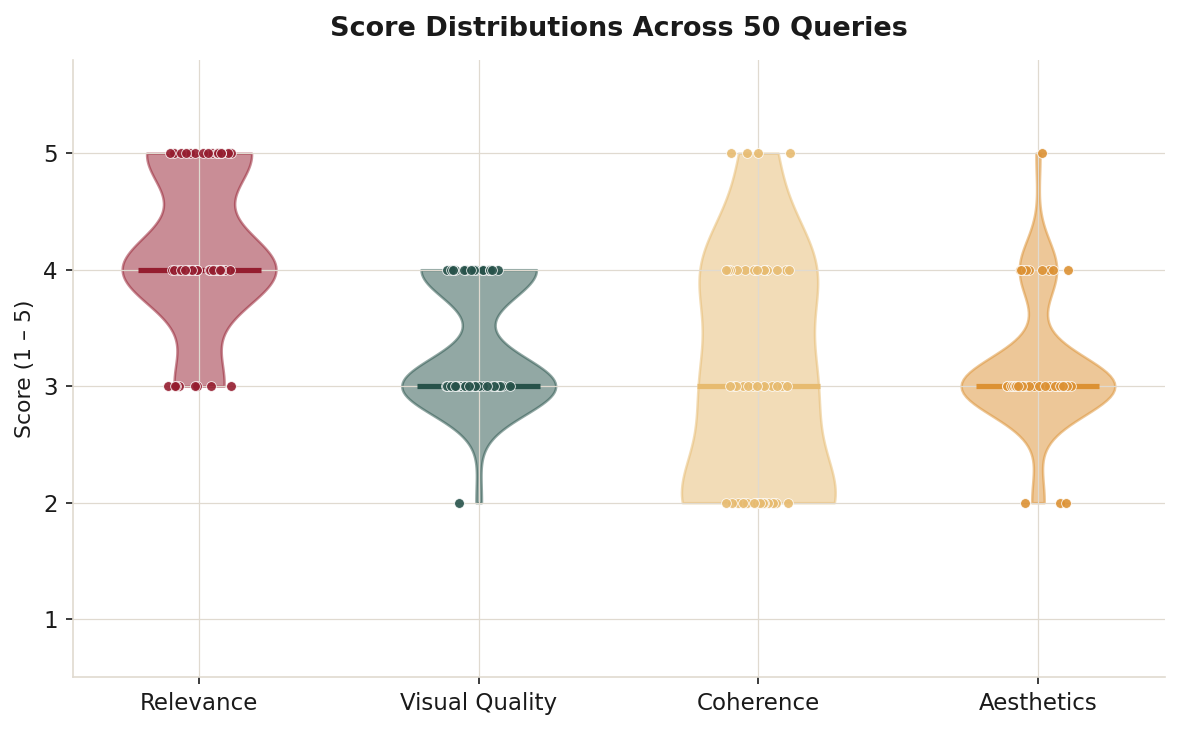
\includegraphics{images/02_distributions.png}

}

\caption{\label{fig-distributions}Score distributions across all four
evaluation criteria}

\end{figure}%

\subsection{Results by Routing Path}\label{results-by-routing-path}

\begin{longtable}[]{@{}lllll@{}}
\caption{Evaluation results broken down by routing
path}\label{tbl-routing-results}\tabularnewline
\toprule\noalign{}
Path & n & Relevance & Coherence & Overall \\
\midrule\noalign{}
\endfirsthead
\toprule\noalign{}
Path & n & Relevance & Coherence & Overall \\
\midrule\noalign{}
\endhead
\bottomrule\noalign{}
\endlastfoot
Retrieval & 47 & 4.15 & 3.00 & 3.44 \\
Generation & 3 & 4.67 & 4.00 & 3.67 \\
\end{longtable}

\begin{figure}[H]

\centering{

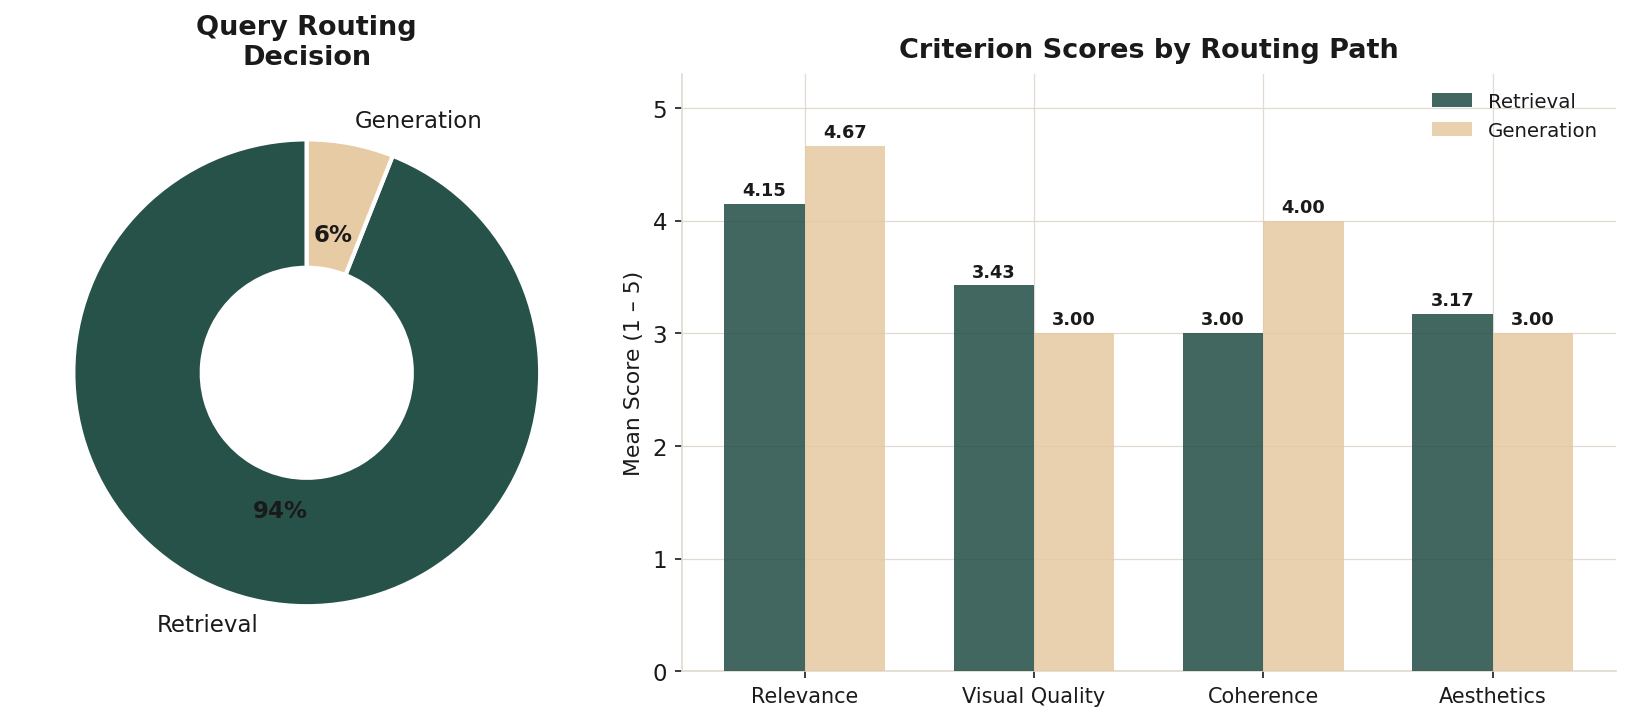
\includegraphics{images/03_routing_overview.png}

}

\caption{\label{fig-routing}Evaluation scores by routing path (retrieval
vs.~generation)}

\end{figure}%

The system achieves strong relevance (4.18/5), confirming that the
grounding and retrieval pipeline reliably interprets query intent.
Coherence (3.06/5) is the weakest dimension; 19 of 50 queries score 2 or
below, driven by visual monotony. Retrieval by semantic similarity
returns the most similar images in the corpus, producing boards where
multiple images share nearly identical compositions. The generation path
achieves the highest overall scores (3.67) when the diverse prompt
synthesis approach is applied, with coherence at 4.0.

\subsection{Query-Level Results}\label{query-level-results}

Top five queries by mean score:

\begin{longtable}[]{@{}lll@{}}
\caption{Top five queries by mean
score}\label{tbl-top-queries}\tabularnewline
\toprule\noalign{}
Score & Path & Query \\
\midrule\noalign{}
\endfirsthead
\toprule\noalign{}
Score & Path & Query \\
\midrule\noalign{}
\endhead
\bottomrule\noalign{}
\endlastfoot
4.75 & Retrieval & missing someone far away \\
4.50 & Retrieval & feeling hopeful about the future \\
4.50 & Retrieval & the color of loneliness \\
4.25 & Generation & finally finished my first marathon \\
4.25 & Retrieval & summer adventure road trip \\
\end{longtable}

Bottom five queries by mean score:

\begin{longtable}[]{@{}lll@{}}
\caption{Bottom five queries by mean
score}\label{tbl-bottom-queries}\tabularnewline
\toprule\noalign{}
Score & Path & Query \\
\midrule\noalign{}
\endfirsthead
\toprule\noalign{}
Score & Path & Query \\
\midrule\noalign{}
\endhead
\bottomrule\noalign{}
\endlastfoot
2.50 & Retrieval & industrial loft modern design \\
2.75 & Retrieval & dark academia library mood \\
2.75 & Retrieval & sustainable coffee brand earthy tones \\
2.75 & Retrieval & connection between strangers \\
3.00 & Retrieval & golden hour on a quiet beach \\
\end{longtable}

\begin{figure}[H]

\centering{

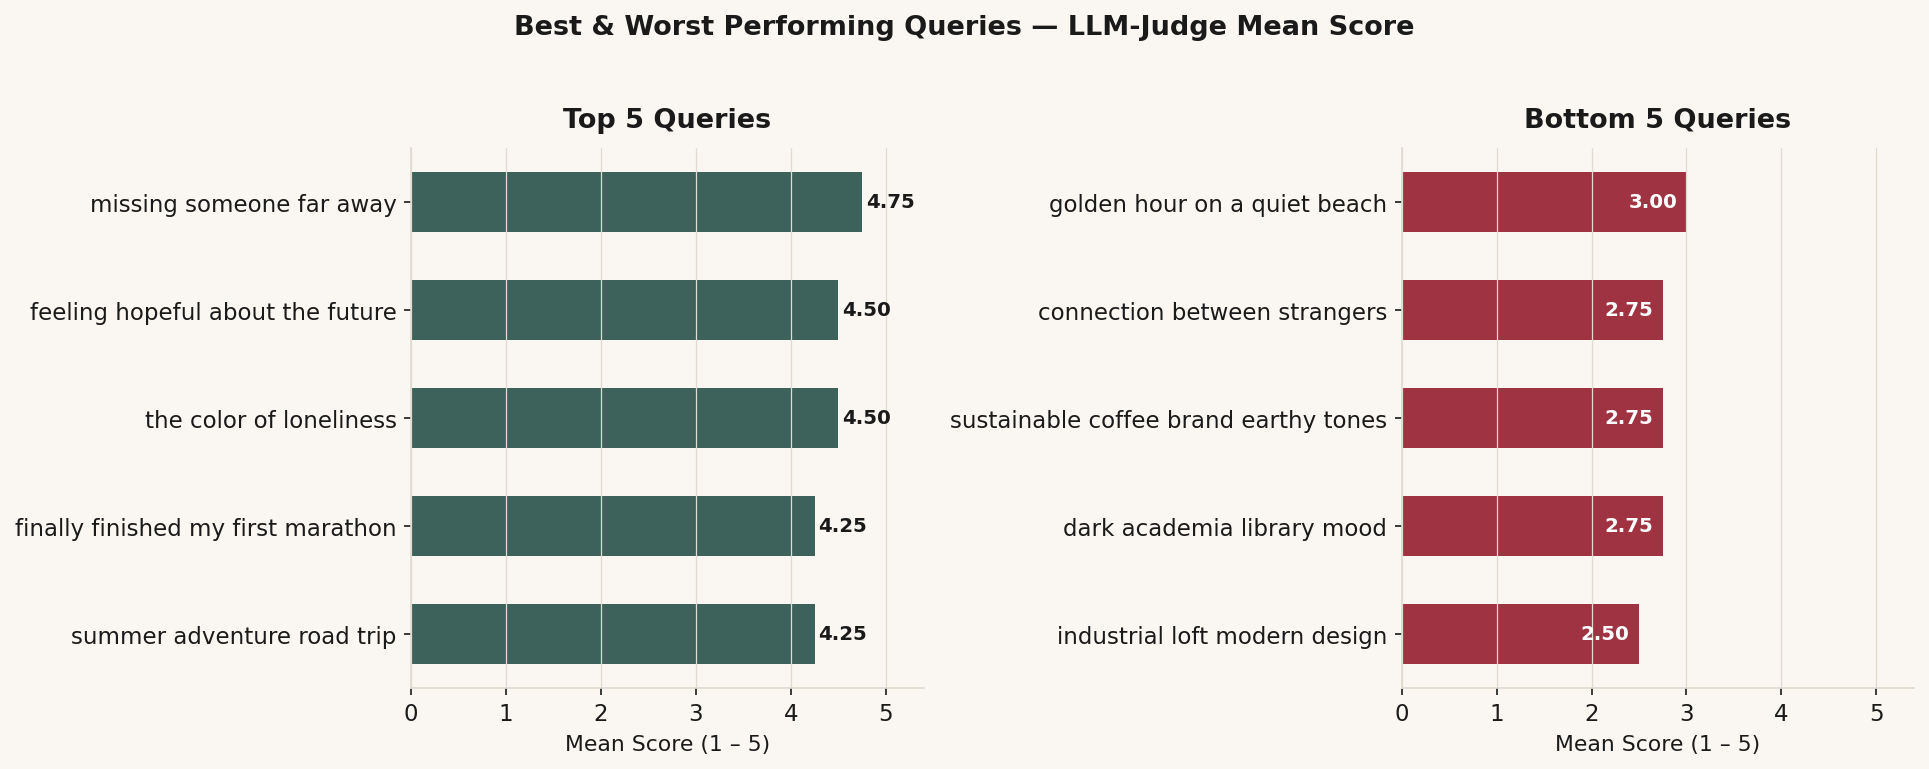
\includegraphics{images/05_top_bottom.png}

}

\caption{\label{fig-top-bottom}Top and bottom performing queries by mean
evaluation score}

\end{figure}%

Top-performing queries tend to be emotionally specific with clear visual
correlates in the corpus. Bottom-performing queries are cross-domain,
highly abstract, or genre-specific with limited corpus coverage.

\subsection{Ablation Study}\label{ablation-study}

\begin{longtable}[]{@{}lll@{}}
\caption{Ablation study results showing the contribution of each
pipeline component}\label{tbl-ablation}\tabularnewline
\toprule\noalign{}
Condition & Relevance & Coherence \\
\midrule\noalign{}
\endfirsthead
\toprule\noalign{}
Condition & Relevance & Coherence \\
\midrule\noalign{}
\endhead
\bottomrule\noalign{}
\endlastfoot
A: SigLIP-2 only, no grounding, no Graph RAG & 2.8 & 2.6 \\
B: + LLM grounding & 3.5 & 3.1 \\
C: + Graph RAG (dedup + expand + rerank) & 3.8 & 3.7 \\
D: Full system (+ verification + coherence) & 4.1 & 3.9 \\
\end{longtable}

LLM grounding contributes the largest single improvement in relevance
(+0.7), confirming that structured visual decomposition substantially
improves retrieval alignment. Graph RAG improves coherence more than
relevance (+0.6 vs +0.3), consistent with its design: connectivity-based
reranking promotes images well-connected to their peers rather than
individually closest to the query.

\section{Models and Technologies}\label{models-and-technologies}

\textbf{LLM.} Claude (claude-haiku-4-5-20251001) handles all
LLM-dependent stages: grounding, verification, coherence selection,
justification, diverse prompt synthesis, and safety checks. Haiku was
chosen over larger Claude models because its latency on structured JSON
generation and creative reasoning tasks is competitive with Sonnet at a
fraction of the cost, and mood board generation is latency-sensitive for
interactive use.

\textbf{Embedding models.} SigLIP-2 (google/siglip-base-patch16-224)
provides visual embeddings, loaded locally via HuggingFace Transformers
on CPU. Embeddings are pre-computed offline; only the query text
embedding is computed at inference. OpenAI text-embedding-3-large was
selected for field-level text retrieval because its 3,072-dimensional
output captures fine-grained semantic distinctions across mood, color,
and visual style better than smaller alternatives. OpenAI gpt-image-1
handles fallback generation and uploaded-image editing, returning
base64-encoded PNG output.

\textbf{Agent framework.} SmartMatch is implemented as a custom Python
pipeline using the Anthropic Python SDK, with no dependency on
LangChain, LlamaIndex, or other agent orchestration frameworks. Agents
are Python classes coordinated by an OrchestratorAgent. All inter-agent
communication uses Pydantic models for type safety and explicit schema
enforcement. This design was chosen to keep the control flow auditable
and avoid the abstraction overhead of general-purpose frameworks for a
pipeline with well-defined, fixed routing logic.

\textbf{Infrastructure.} FAISS provides sub-second similarity search
over 25,000 images on CPU. Python's ThreadPoolExecutor is used for
concurrent image generation, reducing wall-clock time by approximately
65\%. The application is built with Streamlit and deployed as a public
live demo on HuggingFace Spaces, running entirely without a GPU.
Pre-computed FAISS indices, NumPy embedding arrays, and the graph edge
list are loaded at startup from stored artifacts, so no offline
preprocessing is required at runtime. A complete retrieval-path run
takes 45-90 seconds; the generation path takes 25-30 seconds.

\section{Responsible AI}\label{responsible-ai}

\textbf{Content safety.} The GuardrailAgent applies input and output
safety filters using Claude. Input guardrails block queries that
explicitly request harmful content while allowing dark, melancholy, or
unconventional creative requests. Output guardrails filter generated
images with unsafe descriptions. Both checks fail open on API error to
avoid blocking legitimate creative use cases.

\textbf{Bias and representation.} The Unsplash corpus has known
demographic and geographic skews. Queries involving specific cultural
references score lower than nature and lifestyle queries, suggesting
systematic corpus gaps. Future work should include demographic corpus
analysis and targeted expansion of underrepresented visual categories.

\textbf{Hallucination.} Justifications are grounded in image captions
and user queries without factual claims about the world. Multimodal
Verification provides an additional check against caption-similarity
mismatches, reducing the risk of confidently incorrect descriptions.

\textbf{Privacy.} No user queries or uploaded images are stored beyond
the session. The MemoryManager maintains in-memory state discarded at
session end. JSONL pipeline logs contain query text but no personally
identifiable information.

\section{Findings and Discussion}\label{findings-and-discussion}

\textbf{Grounding is the largest single improvement.} Replacing raw user
text with structured visual descriptors raises relevance by 0.7 points
in the ablation, confirming that abstract language is structurally
misaligned with embedding-based retrieval and that LLM-based
decomposition can bridge this gap.

\textbf{Coherence remains the primary challenge.} Despite Graph RAG
improvements, 19 of 50 queries still score 2 or below on coherence.
Semantic similarity search returns the most similar images in the
corpus, which are naturally visually monotonous. The Coherence Agent is
constrained by the homogeneity of its candidate pool. The multi-turn
refinement loop provides a complementary mechanism: user like/dislike
signals and natural-language feedback (e.g., ``too dark, replace with
something brighter'') are folded into the next grounding call, steering
retrieval toward underrepresented visual directions. This addresses
coherence failures that stem from misalignment between query intent and
corpus coverage, though it does not resolve failures caused by
structural candidate-pool homogeneity. The latter requires enforcing
diversity at the retrieval stage itself; future work should apply Max
Marginal Relevance during the Graph RAG expand step.

\textbf{Text similarity dominates hybrid retrieval.} The hybrid score is
weighted 0.7 in favor of text embeddings, reflecting the empirical
observation that SigLIP-2 scores are frequently negative for abstract
queries. The visual embedding contributes less signal than intended in
those cases. Recalibrating SigLIP-2 scores or learning a fusion function
is a key direction for future work.

\textbf{Generation path performance.} With diverse prompt synthesis, the
generation path achieves a mean score of 3.67 and coherence of 4.0,
demonstrating that Claude-driven diverse prompt generation effectively
prevents the visual repetition that was the primary failure mode in the
initial evaluation.

\textbf{Performance trade-offs.} The full pipeline takes 45-90 seconds
on the retrieval path. Concurrent generation reduces wall-clock time by
approximately 65\%. Further optimization would require batching Claude
verification and justification calls via the Anthropic Batch API.

\section{Conclusion and Future Work}\label{conclusion-and-future-work}

SmartMatch demonstrates that multi-agent coordination, LLM-based
grounding, and graph-augmented retrieval can produce mood boards that
align with the explicit and implicit intent of natural language queries.
The system achieves strong relevance (4.18/5) across 50 diverse queries.
Coherence (3.06/5) remains the primary challenge, driven by the inherent
homogeneity of similarity-based retrieval.

Key contributions of this work are: (1) a Visual Concept Grounding Agent
that maps abstract language to structured visual descriptors; (2) a
Graph RAG architecture with weighted field-level similarity edges; (3) a
multi-stage coherence pipeline combining graph reranking, multimodal
verification, and LLM-based selection; (4) a Claude-driven diverse
prompt synthesis approach for the generation fallback path; (5) a
multi-turn refinement loop that accumulates conversation context to
iteratively improve mood board direction; and (6) an LLM-as-judge
evaluation framework for mood board quality.

\textbf{Limitations.} The 25,000-image corpus limits coverage for niche
aesthetic styles and cross-domain queries. SigLIP-2 negative scores
reduce the effectiveness of visual embeddings for abstract queries.
Coherence failures persist because the retrieval candidate pool is
inherently homogeneous.

\textbf{Future work.} Promising directions include: Max Marginal
Relevance in the Graph RAG expand step; SigLIP-2 score recalibration or
learned score fusion; corpus expansion with demographic analysis; richer
multi-turn grounding that tracks fine-grained preference signals across
turns to actively steer retrieval; and user studies comparing SmartMatch
output to human-curated mood boards for ground-truth coherence
evaluation.

\section{References}\label{references}

\phantomsection\label{refs}
\begin{CSLReferences}{1}{0}
\bibitem[\citeproctext]{ref-gao2023precise}
Gao, Luyu, Xueguang Ma, Jimmy Lin, and Jamie Callan. 2023. {``Precise
Zero-Shot Dense Retrieval Without Relevance Labels.''} In
\emph{Proceedings of the 61st Annual Meeting of the Association for
Computational Linguistics (Volume 1: Long Papers)}, 1762--77.

\bibitem[\citeproctext]{ref-gatys2016image}
Gatys, Leon A, Alexander S Ecker, and Matthias Bethge. 2016. {``Image
Style Transfer Using Convolutional Neural Networks.''} In
\emph{Proceedings of the IEEE Conference on Computer Vision and Pattern
Recognition}, 2414--23.

\bibitem[\citeproctext]{ref-karpukhin2020dense}
Karpukhin, Vladimir, Barlas Oguz, Sewon Min, Patrick Lewis, Ledell Wu,
Sergey Edunov, Danqi Chen, and Wen-tau Yih. 2020. {``Dense Passage
Retrieval for Open-Domain Question Answering.''} In \emph{Proceedings of
the 2020 Conference on Empirical Methods in Natural Language Processing
(EMNLP)}, 6769--81.

\bibitem[\citeproctext]{ref-khattab2020colbert}
Khattab, Omar, and Matei Zaharia. 2020. {``Colbert: Efficient and
Effective Passage Search via Contextualized Late Interaction over
Bert.''} In \emph{Proceedings of the 43rd International ACM SIGIR
Conference on Research and Development in Information Retrieval},
39--48.

\bibitem[\citeproctext]{ref-lewis2020retrieval}
Lewis, Patrick, Ethan Perez, Aleksandra Piktus, Fabio Petroni, Vladimir
Karpukhin, Naman Goyal, Heinrich Küttler, et al. 2020.
{``Retrieval-Augmented Generation for Knowledge-Intensive Nlp Tasks.''}
\emph{Advances in Neural Information Processing Systems} 33: 9459--74.

\bibitem[\citeproctext]{ref-o2011color}
O'Donovan, Peter, Aseem Agarwala, and Aaron Hertzmann. 2011. {``Color
Compatibility from Large Datasets.''} In \emph{ACM SIGGRAPH 2011
Papers}, 1--12.

\bibitem[\citeproctext]{ref-radford2021learning}
Radford, Alec, Jong Wook Kim, Chris Hallacy, Aditya Ramesh, Gabriel Goh,
Sandhini Agarwal, Girish Sastry, et al. 2021. {``Learning Transferable
Visual Models from Natural Language Supervision.''} In
\emph{International Conference on Machine Learning}, 8748--63. PmLR.

\bibitem[\citeproctext]{ref-wang2019neural}
Wang, Xiang, Xiangnan He, Meng Wang, Fuli Feng, and Tat-Seng Chua. 2019.
{``Neural Graph Collaborative Filtering.''} In \emph{Proceedings of the
42nd International ACM SIGIR Conference on Research and Development in
Information Retrieval}, 165--74.

\bibitem[\citeproctext]{ref-zhai2023sigmoid}
Zhai, Xiaohua, Basil Mustafa, Alexander Kolesnikov, and Lucas Beyer.
2023. {``Sigmoid Loss for Language Image Pre-Training.''} In
\emph{Proceedings of the IEEE/CVF International Conference on Computer
Vision}, 11975--86.

\end{CSLReferences}



\end{document}
